The result of various SDN techniques which are used in HPC is presented here

\subsection{Evaluation of flow classification techniques}

In this section, we compare the impact of different flow identification techniques on the SDN algorithm for various applications under full bisection fat-tree and 3-to-1 tapered fat-tree configurations. The evaluation includes performance metrics across application communication time for different applications. To evaluate the flow detection technique, we kept the routing fixed as SDN‑optimal and used communication‑computation phase detection, while varying the flow detection methods.

\subsubsection{Performance Under full bisection fat-tree}
\begin{figure}[h]
  \centering
  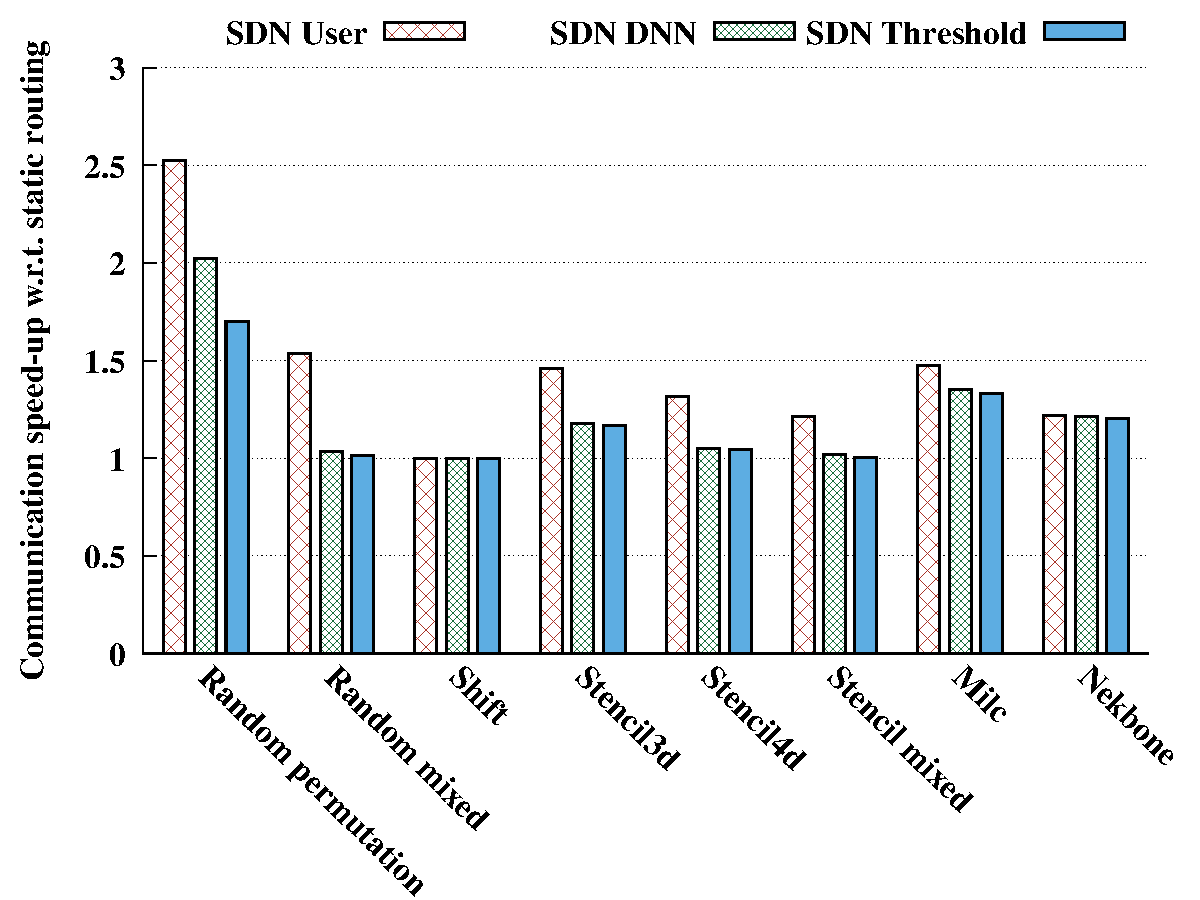
\includegraphics[width=\columnwidth]{./figs_4/full_fat_flow_detection.pdf}
  \caption{Comparison of flow detection in full bisection fat-tree of 1024 nodes}
  \label{fig:fld_full}
\end{figure}

The Figure ~\ref{fig:fld_full} compares communication speedup achieved by three flow detection techniques, SDN User, SDN DNN, and SDN Threshold across various applications, including Random-Permutation, Random-mixed Shift, Stencil3D, Stencil4D, Stencil-mixed, Milc, and Nekbone. These applications represent diverse traffic patterns, ranging from simple to highly complex workloads, making them ideal benchmarks for evaluating network performance.  A higher bar (speedup) signifies better efficiency and lower communication time relative to the baseline. The user flow identification technique performs best due to early flow identification, enabling prompt traffic management. DNN detection ranks second, limited by a 0.3-millisecond delay. Threshold detection performs worst due to delayed flow recognition. Importantly, all three techniques perform better than the widely used single-path static routing, demonstrating the effectiveness of dynamic flow detection in improving communication efficiency within SDN frameworks. User detection consistently leads across all applications. DNN detection shows reasonable gains despite initial delay. Threshold detection offers minimal improvement. These results highlight the importance of incorporating flow detection mechanisms to enhance SDN routing performance beyond conventional static routing methods like D-mod-K, also, the DNN model does a faster flow classification compared to threshold based model without losing in performance.


\begin{comment}
\begin{figure*}[t]
  \centering
  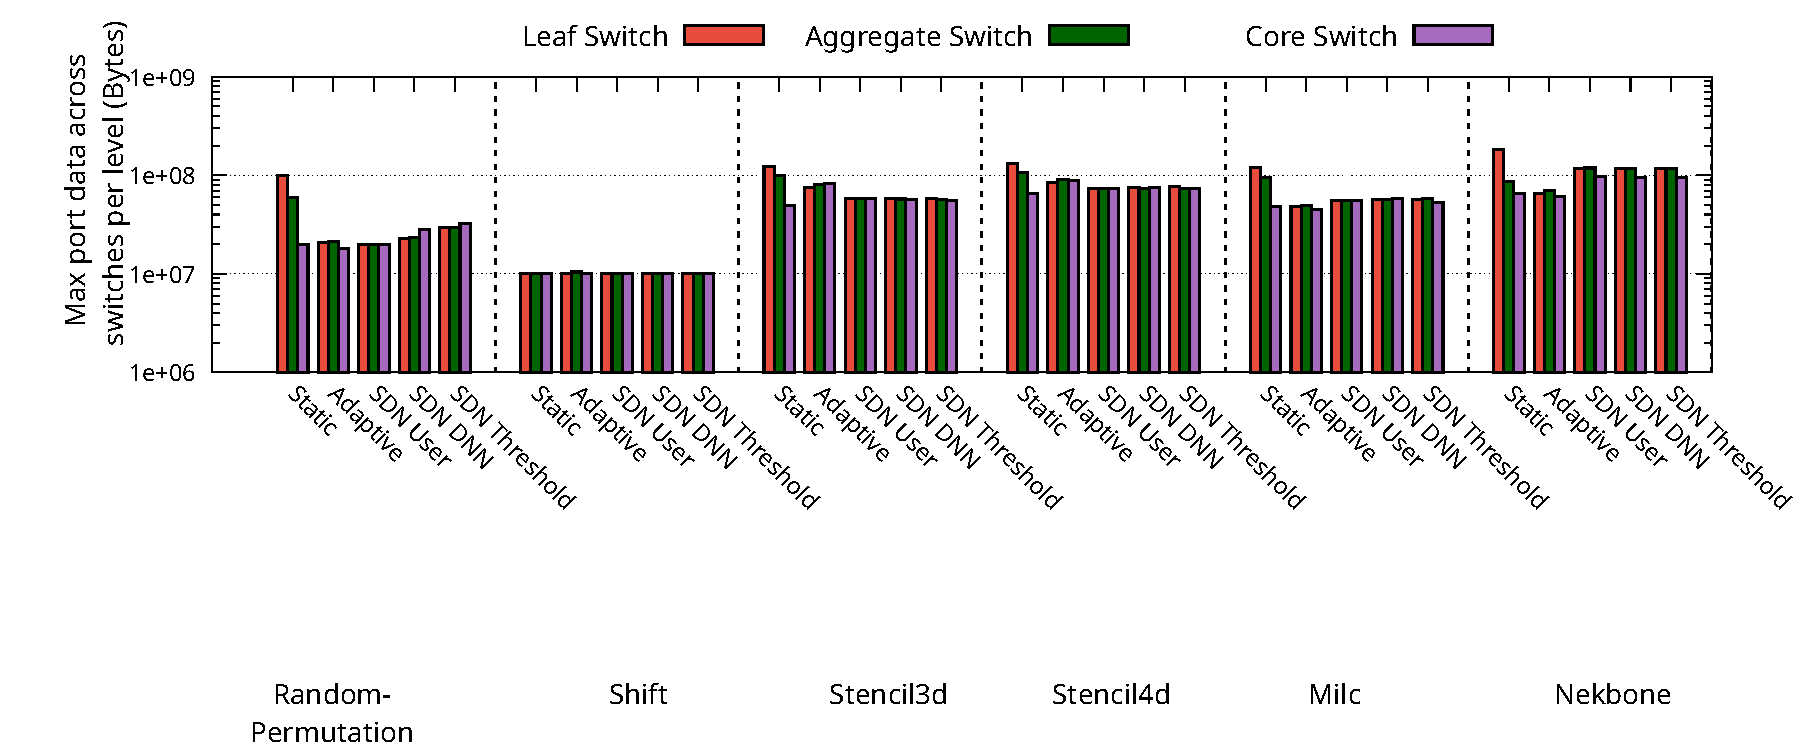
\includegraphics[width=\textwidth]{./figs_4/combined_max_load_plot_full.pdf}
  \caption{Max data sent through a port in a switch level for all switches in full bisection fat-tree of 1024 nodes}
  \label{fig:ld_full}
\end{figure*}



The Figure ~\ref{fig:ld_full} shows maximum outgoing data (Bytes) through ports across six application sections: Random-Permutation, Shift, Stencil3D, Stencil4D, MILC, and Nekbone. Each section contains bars representing three configurations:
Green represents the maximum load at the leaf switches, Blue indicates the maximum load at the aggregate switches, and Red signifies the maximum load at the core switches. Observations reveal that the Random-Permutation application shows the highest load at the leaf switch under the Static configuration. Similarly, Stencil3D and Stencil4D exhibit high loads at both leaf and aggregate switches in Static and Adaptive configurations. Nekbone records the highest outgoing data, particularly at the leaf switch under the Static configuration. When comparing SDN loads, they are consistently lower than those in Static configurations and remain lower than Adaptive configurations when communication density is moderate, as observed in applications like Random-Permutation, Shift, Stencil3D, and Stencil4D. SDN effectively distributes loads across ports, resulting in a positive speedup over static routing.
\end{comment}

\subsubsection{Performance under 3-to-1 tapered fat-tree}
\begin{figure}[h]
  \centering
  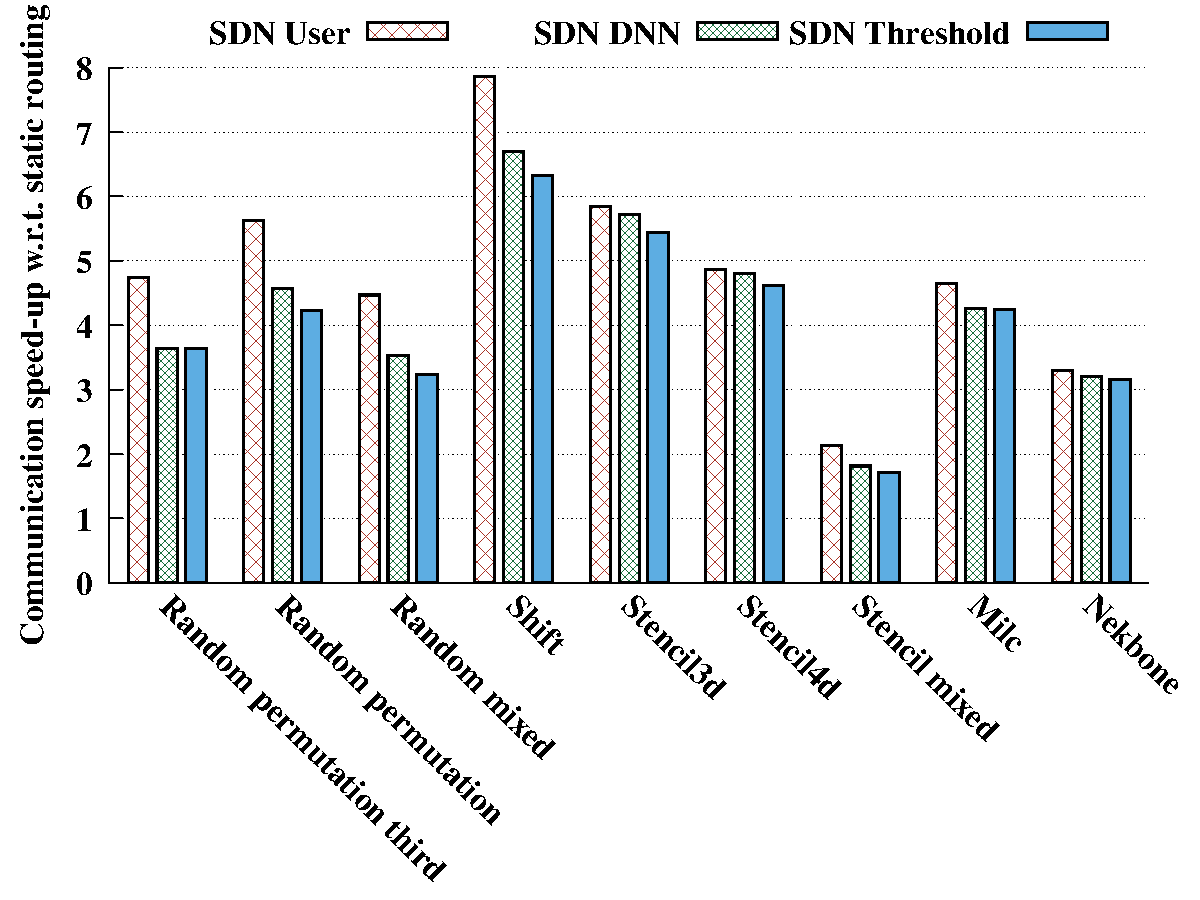
\includegraphics[width=\columnwidth]{./figs_4/taper_fat_flow_detection.pdf}
  \caption{Comparison of flow detection in 3 to 1 taper fat-tree of 1536 nodes}
  \label{fig:fld_taper}
\end{figure}

The Figure ~\ref{fig:fld_taper} illustrates the communication speedup achieved by different flow detection techniques (SDN User, SDN DNN, and SDN Threshold) under a 3-to-1 taper fat-tree topology with 1536 nodes and a 3:1 tapering ratio. This topology emphasizes the impact of reduced bandwidth at higher levels of the fat-tree structure.


In a 3-to-1 tapered fat-tree topology, even a random-permutation pattern represents a relatively dense communication workload. To better demonstrate the effectiveness of our routing mechanism in balancing traffic, we introduced Random-Permutation-Third by removing two-thirds of the communication from a random-permutation of 1536 nodes, retaining only eight out of the 24 communication flows passing through a leaf router. Our evaluation revealed that SDN User consistently achieved the highest speedup, exceeding 6x, highlighting the benefits of early user-provided flow identification that enables optimal traffic balancing from the start. In contrast, SDN DNN and SDN Threshold exhibited moderate speedups of approximately 1.5x and 1.2x, respectively, due to delayed flow detection. Similar trends were observed in the Shift application, where SDN User maintained its superior performance, while SDN DNN and SDN Threshold provided moderate improvements over static routing. In compute-heavy applications such as Milc and Nekbone, the performance gap between techniques narrowed, though SDN User remained the top performer. The results suggest that compute-heavy traffic benefits from steady-state optimizations, though early flow detection consistently outperformed or matched the threshold-based approach. These findings underscore the critical role of early flow detection in achieving optimal traffic balancing, particularly in tapered fat-tree topologies with constrained bandwidth, as reflected by higher speedup values relative to baseline D-mod-K routing.


\begin{comment}
\begin{figure*}[t]
  \centering
  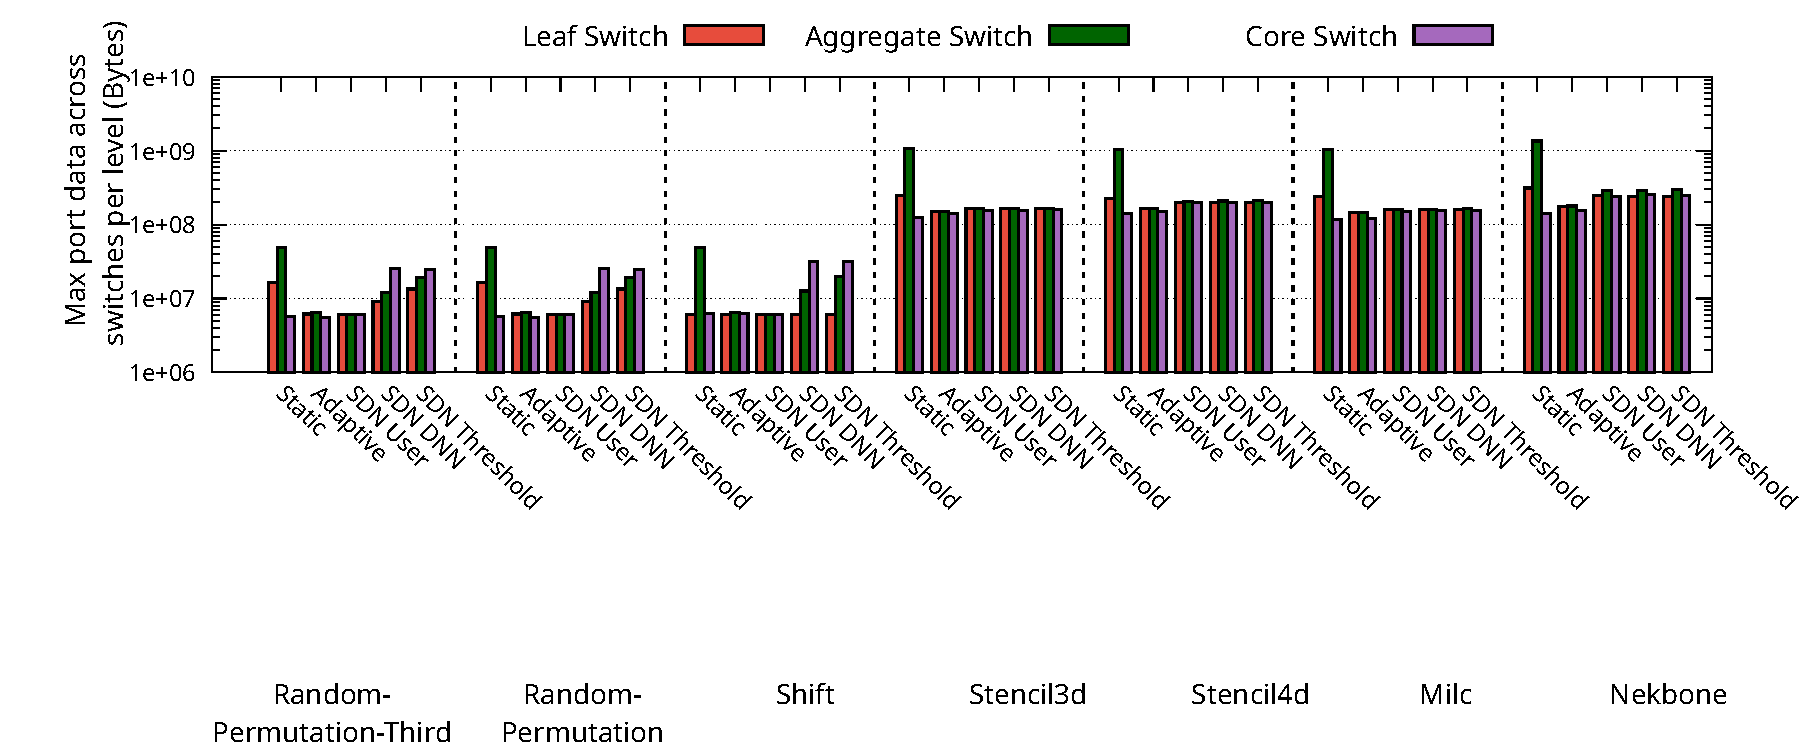
\includegraphics[width=\textwidth]{./figs_4/combined_max_load_plot_taper.pdf}
  \caption{Max data sent through a port in a switch level for all switches in 3-to-1 taper fat-tree of 1536 nodes}
  \label{fig:ld_taper}
\end{figure*}


In tapered fat-tree, the aggregate switch ports have a lot of load, and in all cases, SDN with all various flow identification techniques have always drtibuted this load across the the other switch ports. SDN performance in load distribution is almost same as adaptive and in cases for Shift and Random-Permutation-Third it is doing a slightly better job than adaptive.



%
%
%
%
%
%          next Sub Section 2 of results
%
%
%
%
%

\end{comment}

\subsection{Evaluation of Phase Identification}
This section evaluates the effectiveness of phase identification, across varioous applications under full bisection fat-tree and 3-to-1 tapered fat-tree configurations. To evaluate the communication‑computation phase identification technique, we kept the routing fixed as SDN‑optimal and used the SDN user flow detection method, while varying the phase identification methods.

\subsubsection{Performance under full bisection fat-tree}


\begin{figure}[h]
  \centering
  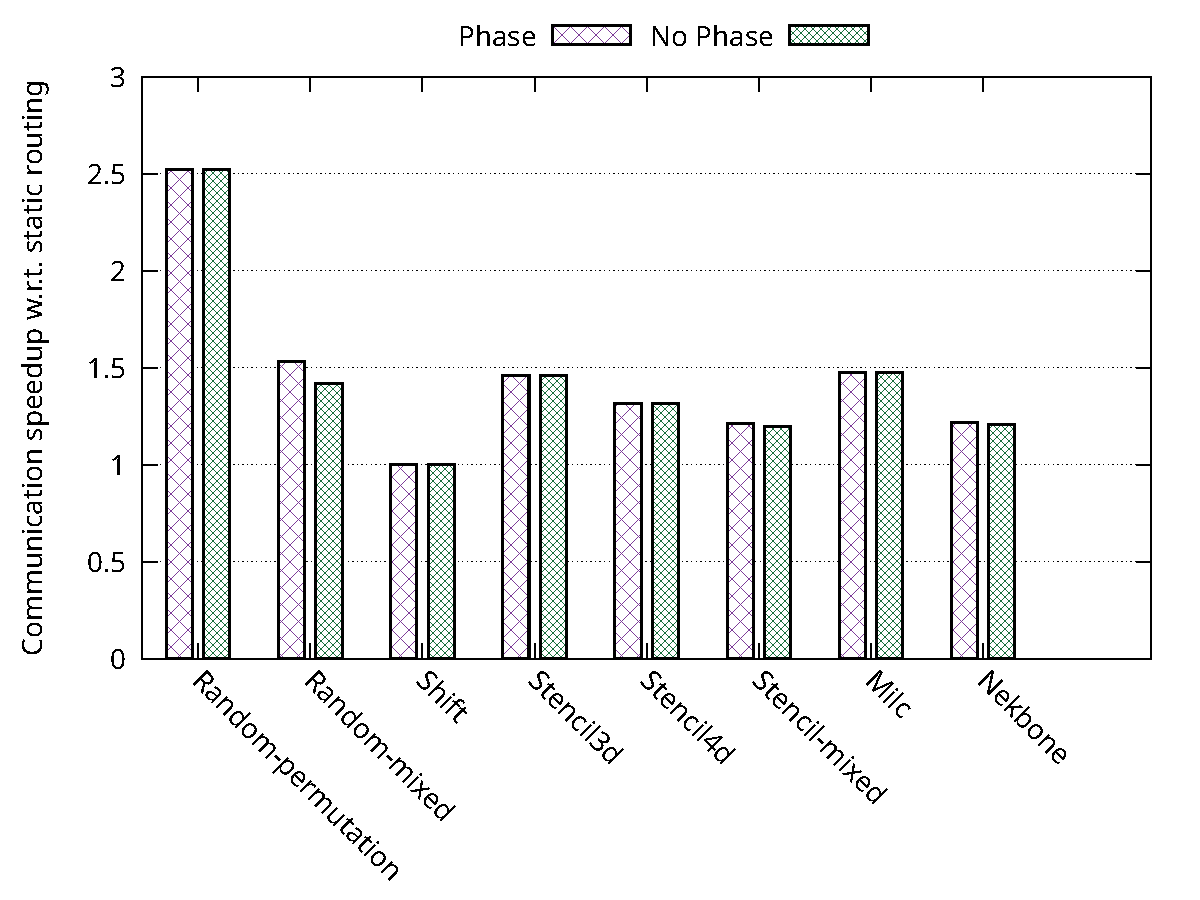
\includegraphics[width=\columnwidth]{./figs_4/phase_full.pdf}
  \caption{Comparison of phase identification in full bisection fat-tree of 1024 nodes}
  \label{fig:phase_full}
\end{figure}
The Figure~\ref{fig:phase_full} shows phase identification results for full fat-tree, where the x-axis represents different workloads, including Random-permutation, Random-mixed, Shift, Stencil3d, Stencil4d, Stencil-mixed, Milc, and Nekbone, while the y-axis quantifies the relative speedup. 
In full bisection fat-tree routing, phase-based optimization leverages threshold-based flow classification and SDN routing to improve communication efficiency. The analysis of communication speedup reveals notable improvements in random-mixed, stencil-mixed, and nekbone, with random-mixed achieving a 7.98\% increase in performance. The phase identification mechanism efficiently distinguishes between different communication phases. When a phase transition occurs, it promptly loads the corresponding routing table, ensuring seamless adaptation to dynamic communication patterns.

The evaluation time for each phase is one-tenth of a polling phase, during which the phase identifier continuously monitors network flows to detect transitions between computation and communication phases. Upon detecting a phase change, it swiftly loads the appropriate routing table to optimize data flow. In random-mixed, stencil-mixed, and nekbone, frequent transitions between computation and communication phases trigger rapid routing table updates, leading to measurable performance improvements in these applications.


\subsubsection{Performance under 3-to-1 tapered fat-tree}
\begin{figure}[h]
  \centering
  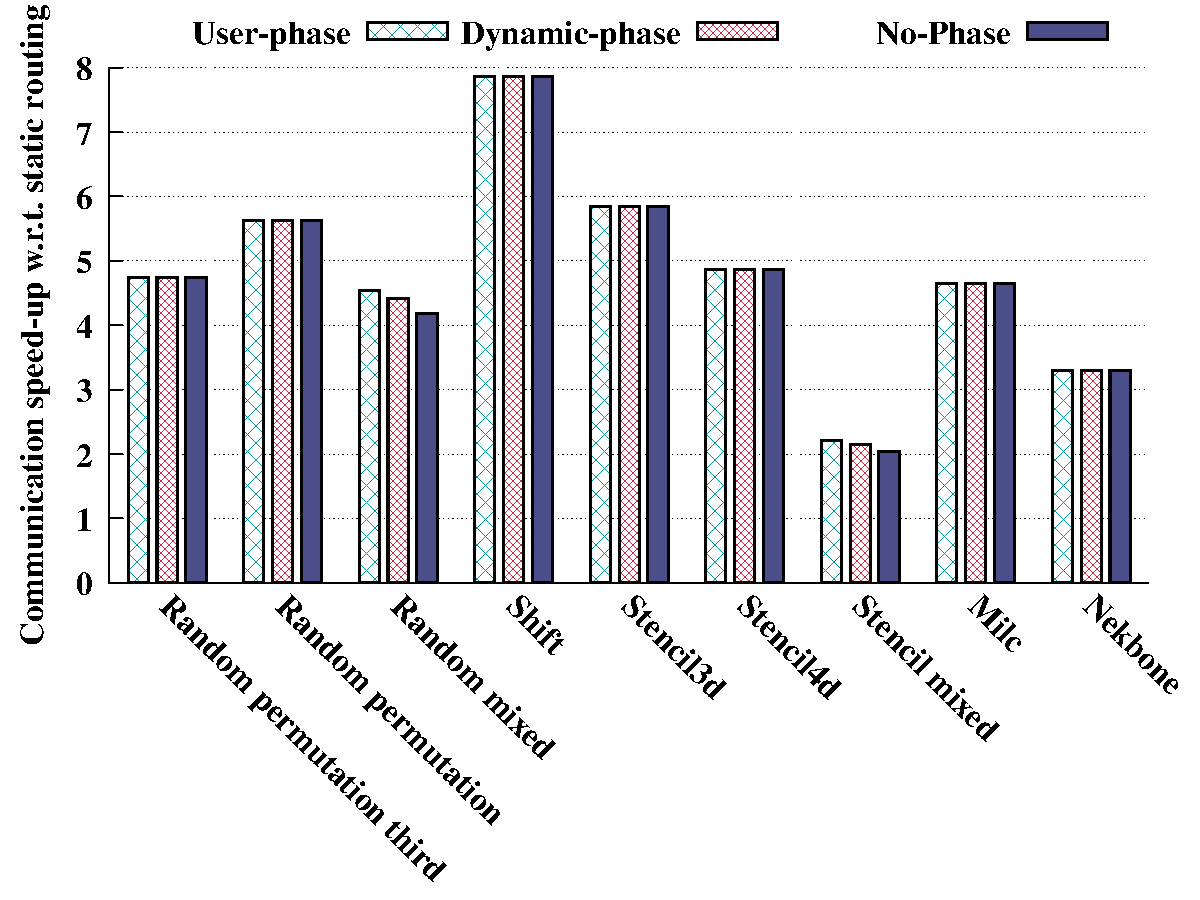
\includegraphics[width=\columnwidth]{./figs_4/phase_taper.pdf}
  \caption{Comparison of phase identification in full bisection fat-tree of 1536 nodes}
  \label{fig:phase_taper}
\end{figure}
The Figure~\ref{fig:phase_taper} shows phase identification results for full bisection fat-tree,
In 3-to-1 tapered fat-tree routing, phase-based optimization dynamically adjusts traffic injection rates using threshold-based flow classification and SDN routing to further enhance communication efficiency. The analysis of communication speedup shows notable improvements in random-mixed, stencil-mixed, and nekbone, with random-mixed achieving an 11.13\% increase in performance, surpassing the gains observed in full bisection fat-tree routing. The phase identification mechanism efficiently detects phase transitions and dynamically manages traffic flow to reduce network congestion

\subsection{Evaluation of SDN-based Routing}
This section evaluates the effectiveness of SDN-based routing approaches across various applications under full bisection fat-tree and 3-to-1 tapered fat-tree configurations of user identification of flows. We analyze performance in terms of communication times.To evaluate the various SDN routing techniques, we kept the communication‑computation phase identification fixed and used the SDN user flow detection method, while varying the SDN routing methods.

\subsubsection{Performance under full bisection fat-tree}
The Figure ~\ref{fig:routing_full} illustrates the communication speedup achieved by three routing techniques—Adaptive, SDN User, and SDN-Adaptive across various applications under a full fat-tree topology. The y-axis represents the speedup relative to static D-mod-K routing, where higher bars indicate better performance.


\begin{figure}[h]
  \centering
  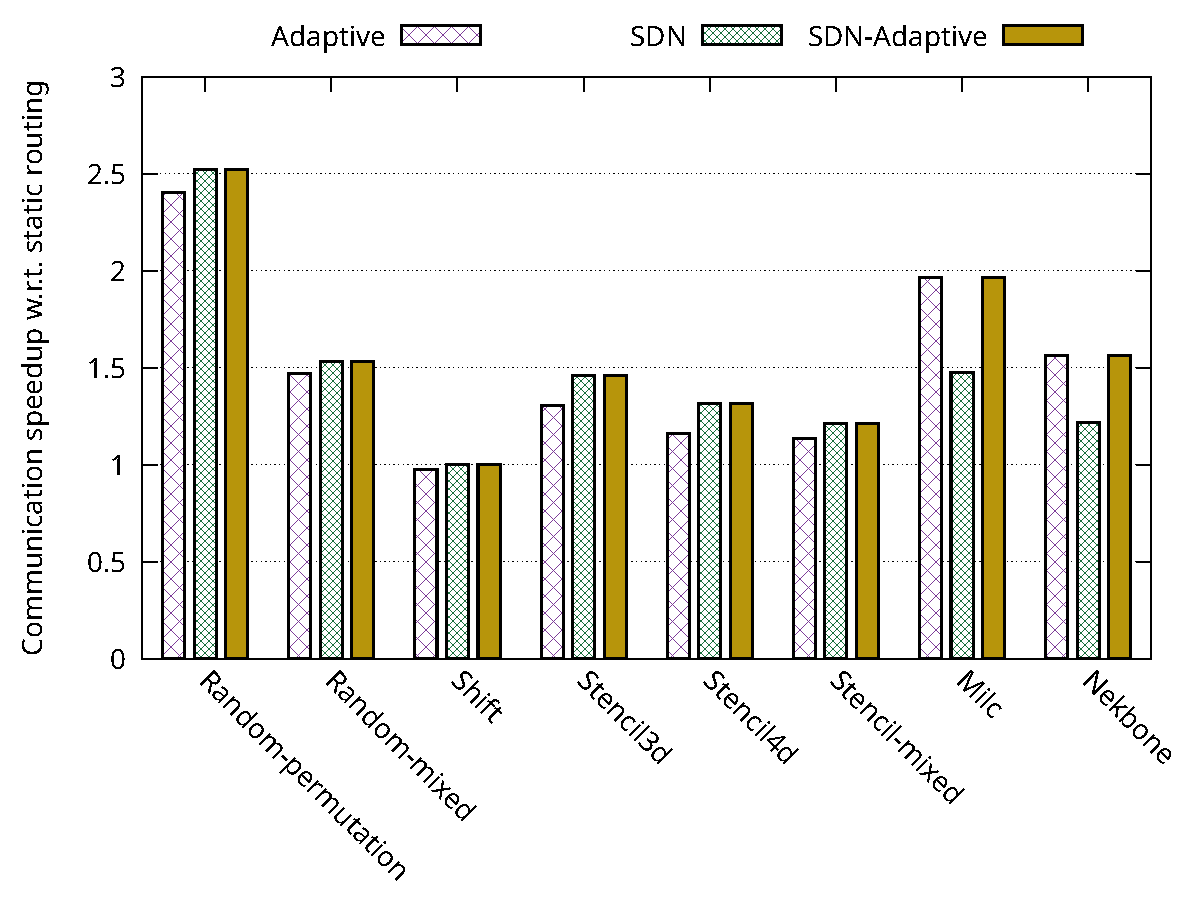
\includegraphics[width=\columnwidth]{./figs_4/routing_full.pdf}
  \caption{Comparison of routing techniques in full fat-tree of 1024 nodes}
  \label{fig:routing_full}
\end{figure}
Single-path SDN routing consistently outperforms single-path DmodK routing across all scenarios.

While SDN routing generally performs better than Adaptive routing, the multipath nature of Adaptive routing allows it to balance the load more effectively when communication becomes dense. At this point, SDN-Adaptive, a hybrid approach combining SDN and Adaptive strategies, performs similarly to Adaptive routing at high communication density application and similar to SDN then the communication density is low, leveraging its flexibility to adapt based on the application's requirements.

\begin{comment}
\begin{figure}[t]
  \centering
  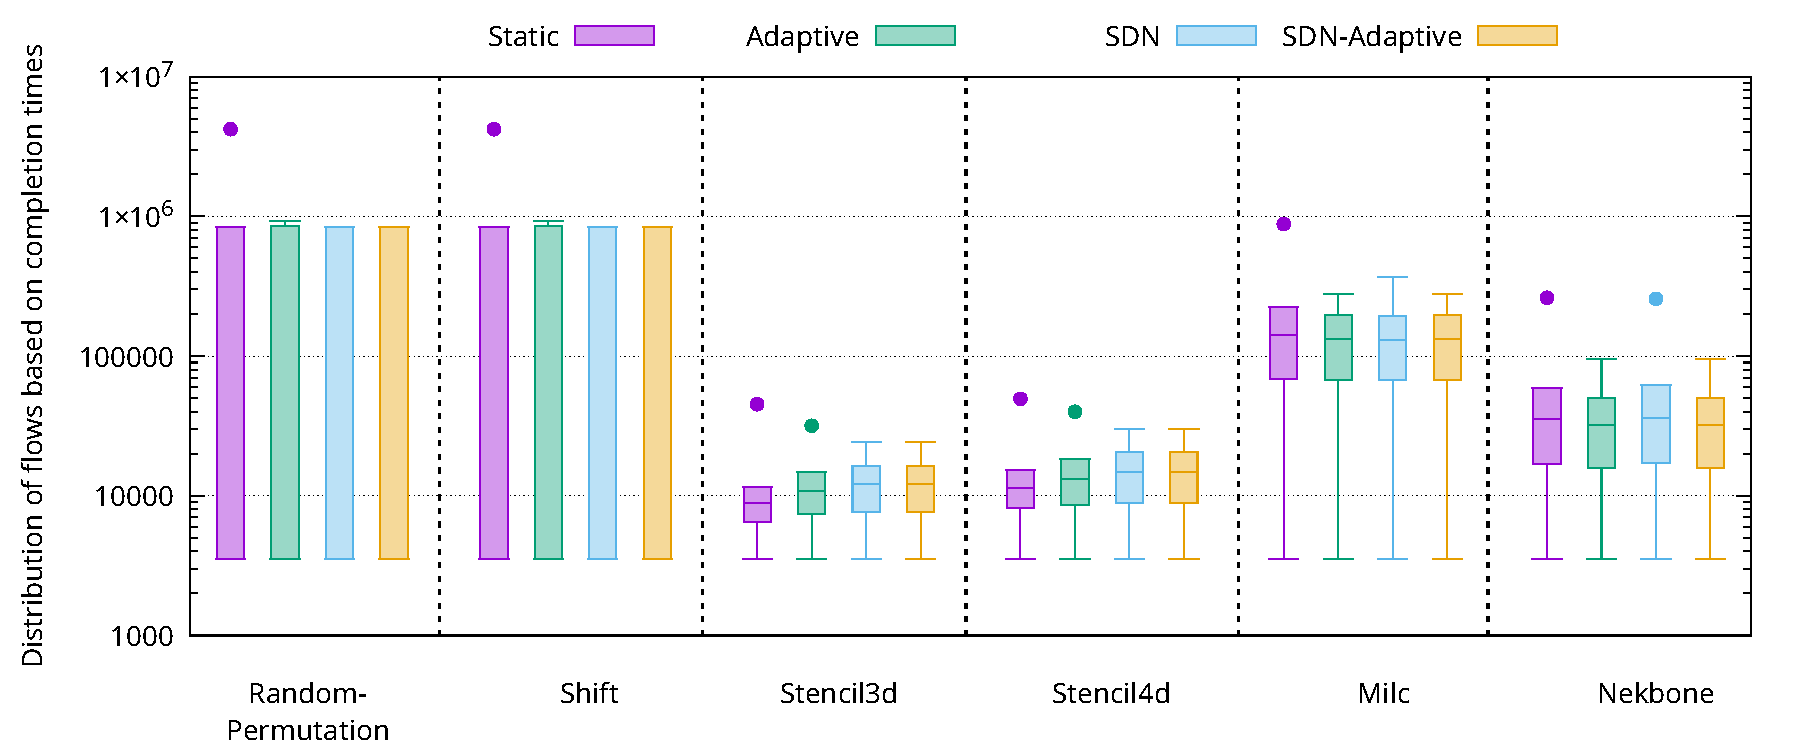
\includegraphics[width=\columnwidth]{./figs_4/two_column_multiplot_boxplots_full.pdf}
  \caption{Distribution of flow completion times in full fat-tree of 1024 nodes}
  \label{fig:flow_dist_full}
\end{figure}


The Figure ~\ref{fig:flow_dist_full} show the distribution of distribution of flows based on flow completion times. 
\end{comment}

SDN even being a single path routing is kind of making sure that flows are completing together and there is no stragglers left behind. 


\subsubsection{Performance under 3-to-1 tapered fat-tree}



\begin{figure}[h]
  \centering
  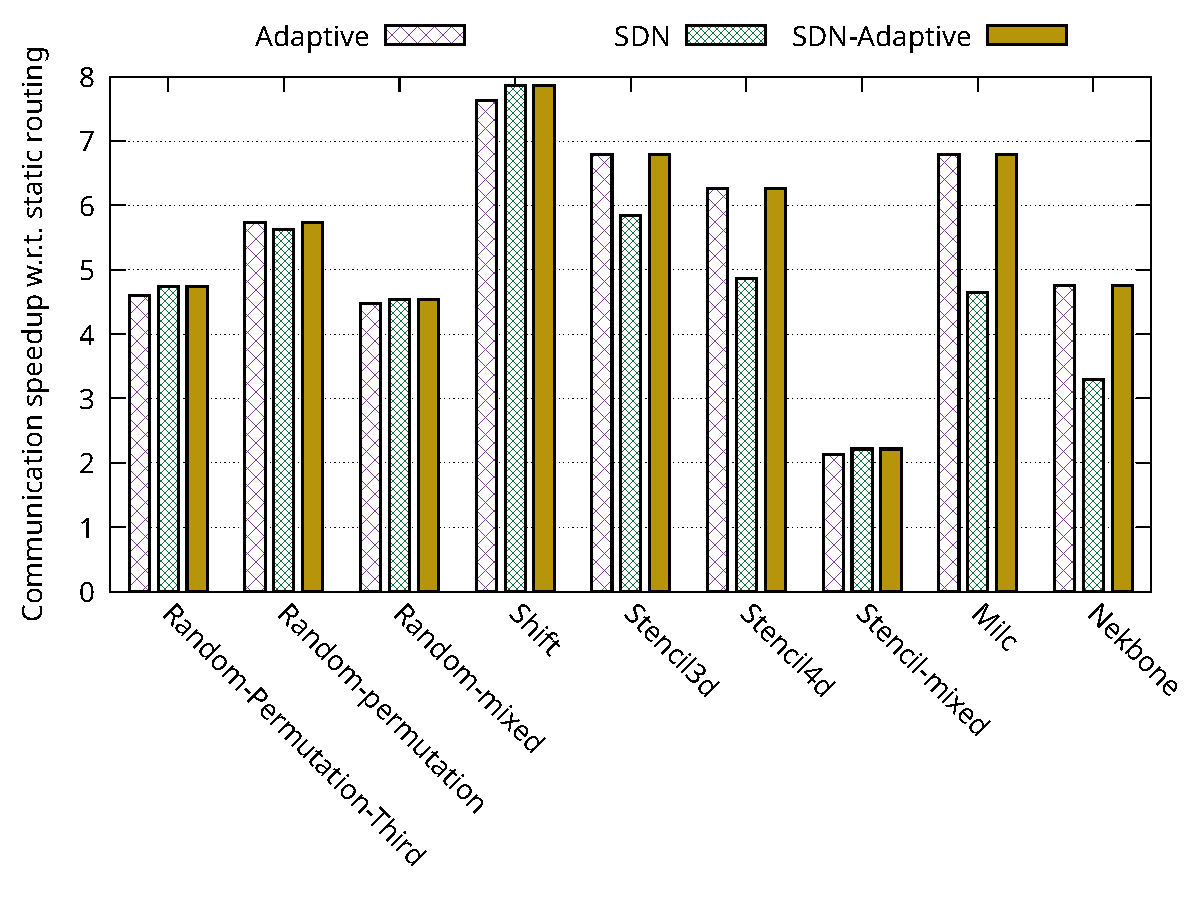
\includegraphics[width=\columnwidth]{./figs_4/routing_taper.pdf}
  \caption{Comparison of routing techniques in 3 to 1 taper fat-tree of 1536 nodes}
  \label{fig:routing_taper}
\end{figure}


The Figure ~\ref{fig:routing_taper} presents a comparison of routing techniques (Adaptive, SDN User, and SDN-Adaptive Use) across three applications (Random-Permutation, Shift, and Milc) under a 3-1o-1 tapered fat-tree topology. The y-axis represents the communication speedup relative to DmodK routing, where higher bars indicate better performance. In a tapered fat-tree topology, applications typically experience dense traffic patterns due to limited bandwidth at higher levels caused by tapering. Adaptive routing demonstrates strong performance in balancing network load, especially under traffic-heavy scenarios. However, in Random-Permutation-Third, where traffic is reduced, our evaluation clearly shows that SDN-based routing outperforms adaptive routing. In Shift traffic patterns, where traffic predictability is higher, Adaptive routing effectively balances the load better than static routing, though SDN-based routing still makes slightly better decisions due to its global network awareness. SDN-Adaptive routing leverages the strengths of both Adaptive and SDN-based routing by dynamically adapting to application-specific traffic patterns, selecting the most suitable approach for optimal performance. 

\begin{comment}
\begin{figure}[t]
  \centering
  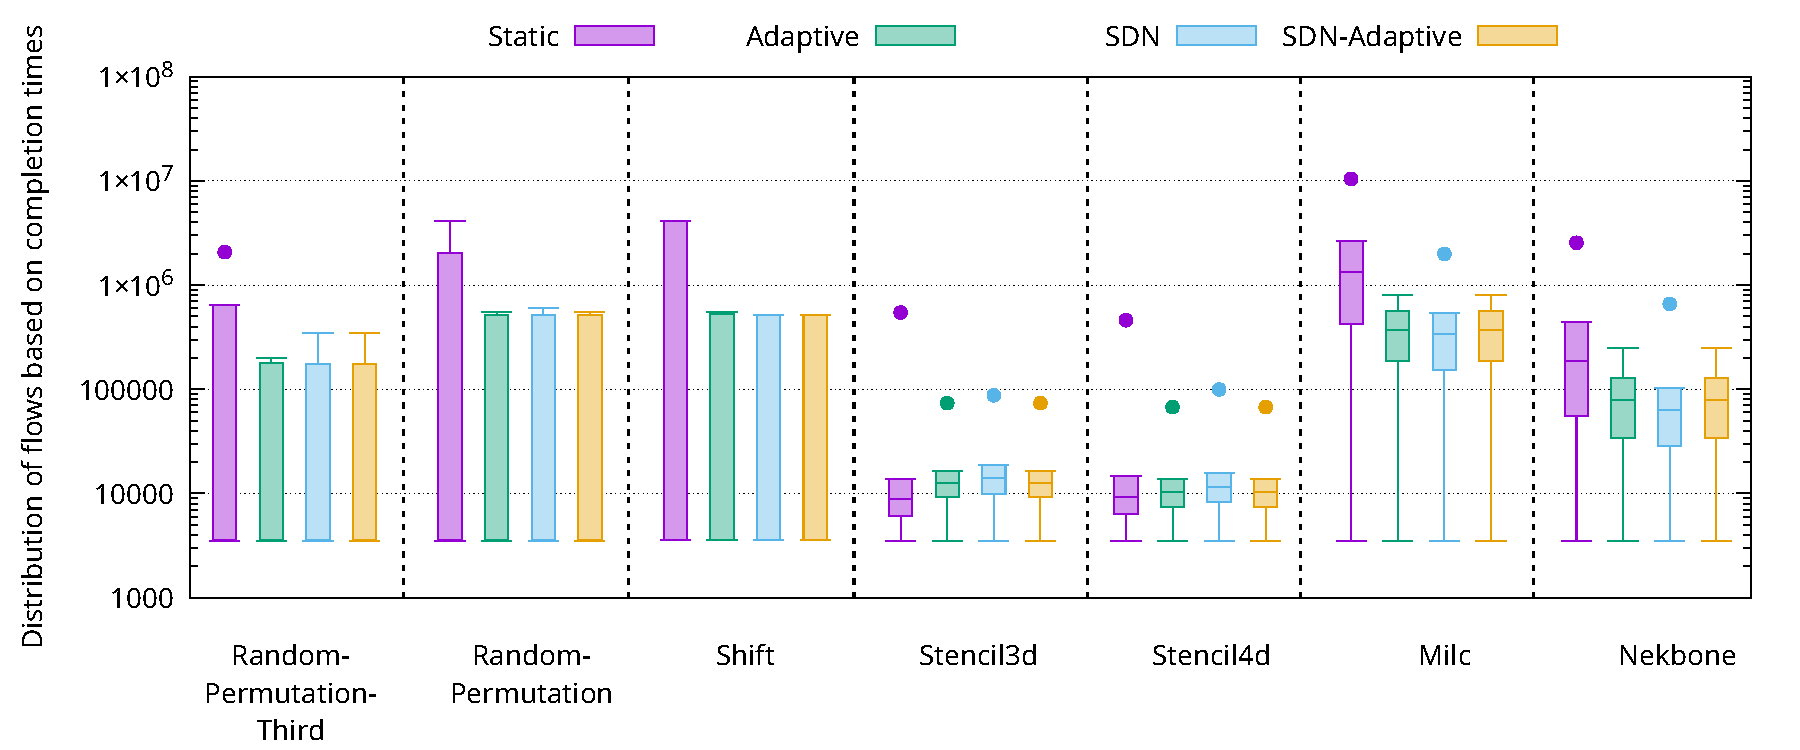
\includegraphics[width=\columnwidth]{./figs_4/two_column_multiplot_boxplots_taper.pdf}
  \caption{Distribution of flow completion times in 3-to-1 taper fat-tree of 1536 nodes}
  \label{fig:flow_dist_taper}
\end{figure}


The Figure ~\ref{fig:flow_dist_full} illustrates the flow completion time distribution. Despite utilizing a single-path routing approach, SDN effectively ensures that flows complete within a similar timeframe, minimizing the presence of stragglers. This highlights the capability of SDN to maintain consistent flow completion, reducing delays and enhancing overall network performance.
\end{comment}
